\newpage

\subsection{Schnittstellenbeschreibung und Integration der Komponenten}
\begin{itemize}
    \item Planung der Schnittstellen zwischen den Komponenten
    \item Einfaches Diagramm in DrawIO:
    \begin{itemize}
        \item Zwischen Jonas und Leon: \texttt{downsampleandread1024()}
        \item Zwischen Syzmon und Jonas: \texttt{filemanager struct}, etc.
        \item Zwischen Szymon und Leon: \texttt{filemanager struct}
    \end{itemize}
    
    
    Folgendes Diagramm zeigt die Relation und Interaktion der 4 Komponenten miteinander.
    
    \begin{figure}[H]
    	\centering
    	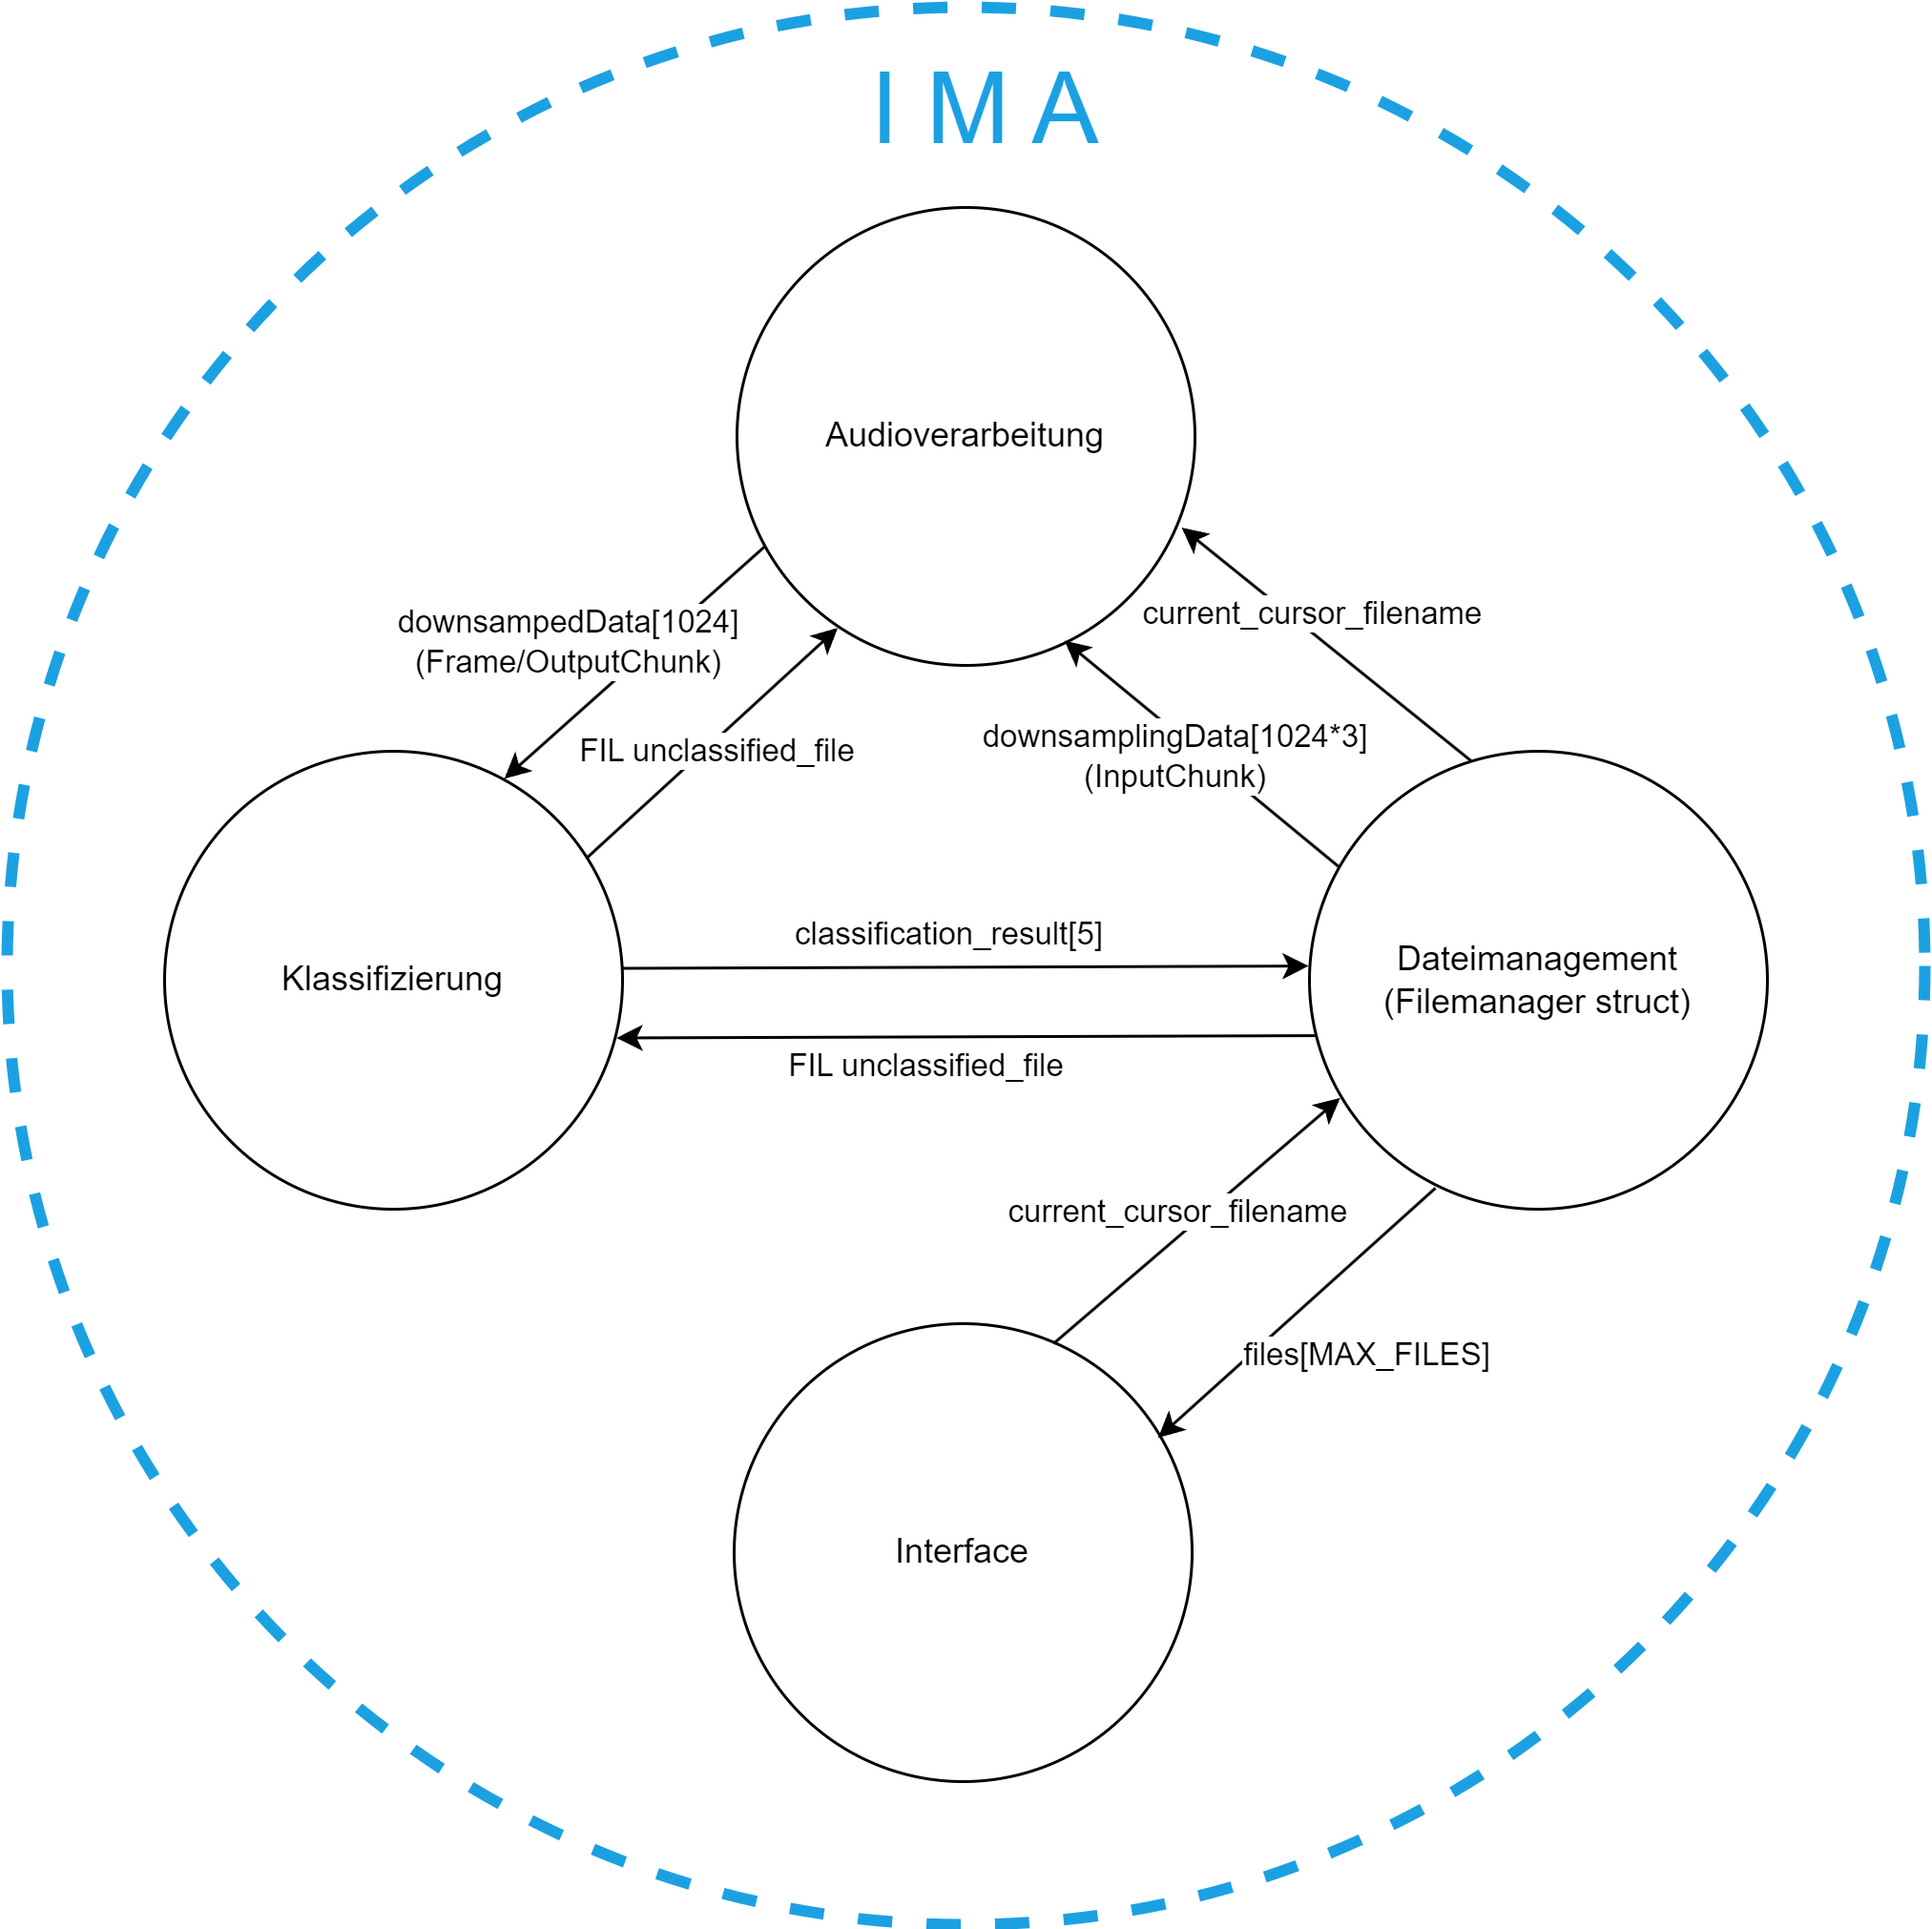
\includegraphics[width=1.0\textwidth]{images/04_spezifikation/komponentendiagramm.drawio.png}
    	\caption{Komponentendiagramm}
    	\label{fig:komponentendiagramm}
    \end{figure}
    
\end{itemize}

Das \textbf{Dateimanagement} ist der zentrale Knotenpunkt des Gesamtsystems. Es dient zunächst als Zugriffspunkt auf die Samples anhand ihrer Namen. 

Beim Hinzufügen neuer \textbf{Samples} in das \textbf{Dateisystem} werden diese zunächst als \boldinline{unclassified_file Fil} an die \boldinline{Klassifizierung} übergeben. Dieser wird an die Audioverarbeitung weiter gegeben.\textbf{TODO: Beschreibe die Übergabe der Downsampling Daten.}

Die für das Spektrogramm benötigten heruntergesampelten Daten werden zur \textbf{Klassifizierung} weitergeleitet. Basierend auf dem Spektrogramm werden die Dateien anhand ihrer Klangmerkmale klassifiziert. Die Ergebnisse dieser Klassifikation werden in \boldinline{classification_result[5]} gespeichert. Dieses Array wird anschließend an das Dateimanagement übergeben und wird dem Sample zugeordent.
 
Das Interface ruft alle Dateien aus dem \boldinline{FileManager Struct} in \boldinline{files[MAX_FILES]} ab. Es filtert die Dateien basierend auf den festgelegten Filtereinstellungen und speichert die übereinstimmenden Dateien in \boldinline{shownFiles[MAX_FILES]}.

Beim Auswählen eines Samples wird dessen Name in \boldinline{current_cursor_filename} gespeichert welcher ein Part den \boldinline{FileManager} ist. Die \boldinline{Audioverarbeitung} greift auf diesen Namen zu, um das Sample zu laden und abzuspielen.

